\pagenumbering{arabic}
\chapter{Introduction}
\label{intro}
The chapter outlines an introduction to the subject area of this Final year Project (FYP), the objectives of this project, the methodology used to complete this project, an overview of the report and an explanation of the motivation behind this FYP.

% % \subsubsection*{Promising Approaches of Computer-supported Dietary Assessment and Management: 
% % Current Research Status and Available Applications}
% % \textcite{arens2015promising}
% \textcite{goodman2015vitamin}


\section{Overview}
This project explores identification and classification of food images for use in a calorie measurement android application.
Food calorie consumption is a huge problem in the modern world.
Over 25\% of the population in Ireland is obese and this figure is likely to rise over the coming years.
A mobile application that could help keep track of a user's calorie intake by taking pictures of their meals would be a great help.
The area of computer vision is a very difficult topic to address as it is a very hard task for computers to undertake.
We, as humans, take vision for granted as we can soon see, from the study of computer vision, that there are many difficult steps that have to be made for full identification and classification of an image.

When looking into calorie measurement using an image, there are three questions that have to be answered:
\begin{itemize}
	\item{Where are the Regions of Interest (ROI) in this food image?}
	\item{What food types are in these ROI's?}
	\item{What is the portion size of each food type?}
\end{itemize}

In this project, the main focus will be on the first two questions, 'Where are the
Regions of Interest (ROI) in this food image?' and 'What food types are in these ROI's'. The first step is normally achieved through image segmentation. Image segmentation is the process in which you divide an image into multiple segments as per Figure \ref{fig:imageSeg} and \ref{fig:preImageSeg}.

\begin{figure}
	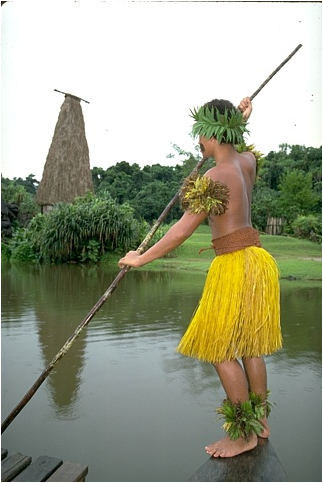
\includegraphics[scale=0.5]{orig}
	\caption{Pre-segmented Image}
	\label{fig:preImageSeg}
\end{figure}

\begin{figure}
	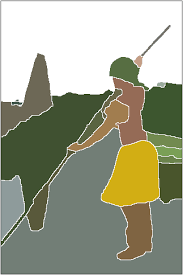
\includegraphics[scale=0.5]{segment}
	\caption{Segmented Image}
	\label{fig:imageSeg}
\end{figure}


Many researchers in various computer vision labs have attempted to solve this
problem using different methodologies.
There has been promising results from some papers but these are mostly under highly constrained circumstances.
When mixed foods are introduced to the problem, many of the methods fail.
Convolutional Neural Networks (CNN) have had very promising results in the field of image classification in the recent years and have been shown to work best is in the area of face detection.

Extensive research on many different methods of image segmentation and classification has been carried out but it seems that CNN's have had the best results for multiple objects in one image and therefore, this method will be applied to many foods in an image.
This is because we will rarely want to classify an image that only has one food
item in it. Therefore, the one shot approach may not be the most successful by which we
build a classifier that takes in an image and gives back the most likely food in
that image. In contrast to this, there could be an element of sub-sampling of the image to rectify this.

The system proposed to solve the problem statement would be able to integrate with an Android mobile phone application. The idea is, that when a user is about to eat their meal, they can simply take a picture of their meal for computation. From here, the application would take an image, and send it to a server to be analysed.
On the server side the image would be classified using a Tensorflow model.
Once this is done, the size of each food type would be measured and through this an overall calorie count would be displayed for the user. This could be logged for user metrics. The full system may not be possible to implement due to time constraints so therefore, classification will be the furthest step looked in to.

\section{Objectives}
\subsection*{Primary Objectives}
\subsubsection*{Use Convolutional Neural Networks for Food Image Classification}
There has been a large paradigm shift in food image recognition in recent years to using convolutional neural networks. This paradigm will be used to answer the problem statement.

\subsubsection*{Tune the CNN, replicating previous work}
There are many different approaches to food identification and classification,
many of which we will see in Chapter 2. An approach will be selected that has
shown promising results in the past and replication of these results will be attempted. In addition to this, there are many different network architectures and parameters that can be adjusted when building CNNs and these will be tuned in order to get the best outcome possible.

\subsubsection*{Develop a mobile application to leverage the CNN}
Another objective for this project is to develop an application that can be used
for dietary assessment. This application would be able to take an image and then send the image to a server to identify and classify the foods within the image. Size estimation will not be explored for this project. Alternatively, a previously developed application will be used to demonstrate the CNN developed.

\subsection*{Secondary Objectives}
\subsubsection*{Understanding of Convolutional Neural Networks}
In the project, Convolutional Neural Networks (CNN's) will be used for object identification in Food Images.
A machine learning library will be used for this due to time constraints but it is a key
objective to develop a deep understanding of CNN's as they are quite pivotal in the current computer vision industry and bio-inspired systems are very interesting.

\subsubsection*{Learn about different image identification and classification techniques}
Although, CNN's will be used for implementation, other methods of identification and classification will not be ignored.
It is very important to learn about other methods as different methods
are better suited for some situations and it would be best to know about these methods due to the inevitability of their use.

\section{Methodology}
The following methodology were adapter for this project:

\subsection*{Define the research question}
The first step to this project was to define the research question.
The general area of a computer vision supported nutritional assessment application was known at conception but the scope of this is too broad for an FYP.
Therefore it was decided that the research question would be to look at the food identification and classification aspect.

\subsection*{Literature Review}
Once the research question was defined, finding related work was the next milestone.
There are many attempts at Food Image Classification and these were not difficult to find, using Google Scholar, but many of these papers glossed over the segmentation aspect and relied on third parties for this step.
Because of this, quite a few references to different papers had to be followed that focused solely on image segmentation and classification.

\subsection*{Explore different image identification methods}
Various image identification methods were collected from the literature review
that was carried out, so there were many options to evaluate.
Convolutional Neural Networks were the clear choice due to recent popularity and successful results, so more traditional methods of identification using colour and texture was not so strenuously explored.

\subsection*{Select an image identification and classification method}
After the various methods to identify and classify food images had been collated in the literature review, one of these had to be selected.

\subsection*{Research technologies and develop skills in these technologies}
As Convolutional Neural Networks (CNN) are used in this project, many resources have been leveraged to enrich understanding of the process.
Tensorflow is the main resource utilised  in creating a CNN so on-line tutorials for this technology were greatly beneficial.
A Deep Learning Course on Udacity was also used to enhance understanding and skills.

\subsection*{Build a prototype of the application}
A prototype application had to built for demonstration for this project.

\subsection*{Compare and analyse results to other implementations}
Once a model had been successfully trained, comparison to previous work was carried out.

\section{Overview of Report}

This report is broken down into various chapters.
The introduction chapter is to give on overview of what this project is about, how the project will be approached and why it is being carried out.
Following this, some information on the background of the subject of this Final Year Project (FYP) will be outlined. Once the chapters of introduction and background have been completed, a chapter outlining the learning of Tensorflow will be explored. Tensorflow is a machine learning library that is used to develop CNNs. In this chapter, the goal is to demonstrate the activities undertaken to learn about the technologies used and show tutorials that have been completed to aid with this learning.
In chapter titled 'Training Using the Inception-V3 Model Architecture' , the purpose is to outline experiments that have been carried out in relation to training Tensorflow models.
A Tensorflow model is the term used to describe the neural network produced by Tensorflow. 
The Inception-V3 architecture is proven to be a very successful architecture for classifying images and will be explained in detail in said chapter.
Once the model has been trained, the following chapter 'Analysing the Trained Model' will consist of experiments that analyse and test the models trained.
A prototype smart phone application was developed to demonstrate the efficacy of the system and an overview of the process will be explained in the chapter titled 'Prototype Application.'
The final chapter's purpose is to provide a discussion on the results obtained and offer a conclusion to the findings.

\section{Motivation}
I find the topic of Computer Vision a very interesting one.
It excites me, to be able to 'teach' a machine how to see as we do.
For this reason, I really wanted to learn about Neural Networks
and this was a large motivator for this project.

Once I had a topic that I wanted to research, I needed a focus or problem statement for this research.
I find that it is much more rewarding to work on something that positively
impacts both myself and other people so I decided that I wanted to research
something that fit this requirement.

Food calorie consumption is a very big problem in the modern world.
Over 25 \% of the population in Ireland are obese.
A mobile application that could help keep track of a user's calorie intake by taking a picture of their meals would be a big help to combat this problem.
This problem statement works very well for me because of it's application use and because of its complexity.
Identifying and recognising food is much more difficult than say recognising faces as it has no uniform shape.
Therefore, this problem would also be very beneficial to developing skills in the computer vision area.

I would like to develop these real world skills so that I can partake in
Computer Vision projects in industry or to do further research in academia. This
is because machine learning has really taken off in the last few years and is
used by many in industry. While machine learning as a whole has become very
popular, computer vision is probably the most prominent that has come out of it.
Face detection, for one, is being researched extensively for use in personalised
advertising and also secure access to devices and systems.
